\documentclass[a4paper]{article}

\usepackage{fancyhdr}
\usepackage{graphicx}
\graphicspath{ {./images/} }

\pagestyle{fancy}
\fancyhf{}
\lhead{Optik und BOS: Wochenaufgabe 4}
\rhead{\today}
\lfoot{HTWG Konstanz}
\rfoot{Seite \thepage}

\begin{document}
	\thispagestyle{empty}
	
	\begin{center}\strut
		\bfseries\Huge
		Wochenaufgabe 4
	\end{center}
	\vfill
	
	\begin{center}\strut
		\textbf{Optik und bildgebende optische Systeme}\\
		Hochschule Konstanz Technik, Wirtschaft und Gestaltung\\
		Wintersemester 2021/22
	\end{center}
	%\vfill
	
	\begin{center}\strut
		\textbf{Team 6:}\\
		Milan Kaiser\\
		Ruwen Kohm\\
		Christian Schmeißer\\
	\end{center}
	\vfill
	\vfill

	\clearpage
	
	\section{Unterschied Farbe - Spektrum}
	\textbf{Schreiben Sie eine kleine Tabelle, wo Sie in dem Sinne der Folien von Farbe sprechen und wo Sie besser vom Spektrum sprechen sollten.}\\
	\begin{center}
	\begin{tabular}{ c|c }
		 & Erklärung \\ 
		\hline
		Spektrum & Ein Spektrum beschreibt eine Menge von Wellenlängen\\
		& und deren Ausprägung.\\
		& Von einem Spektrum ist die Rede \\ 
		& wenn man explizit über Licht (oder andere Wellen) spricht.\\
		\hline
		Farbe & Eine Farbe ist unsere Interpretation eines Wellenlängenspektrums.\\
		& Von Farbe sprechen wir wenn es um die Wahrnehmung von Licht geht.\\
	\end{tabular}
	\end{center}
	\vspace{10pt}
	
	\textbf{Hat eine reife Tomate die Farbe rot? Schreiben Sie einen Satz dazu auf.}\\
	Nein, die Tomate reflektiert nur Licht, welches wir rot wahrnehmen.\\
	
	\textbf{Unter der Definition von Folie 3, beschreiben Sie das, was Sie erleben, mit den Begriffen Farbe und Spektrum}\\
	Unsere Augen nehmen ein Spektrum an verschiedenen Wellenlängen auf und interpretieren dieses als Farbe. Verschieden zusammengesetzte Spektren können zu der selben Farbe führen, da manche Wellenlängen für den Menschen nicht sichtbar sind, oder weil sich manche Farben mischen lassen. Das selbe Spektrum kann auch zu verschieden Farben führen, da unsere Wahrnehmung sehr abhängig von Kontext und Umgebung ist.
	
	\newpage
	
	\section{Wahrnehmung von Spektren}
	\textbf{Skizzieren Sie zwei unterschiedliche Strahlungsspektren, die im Auge die Farbe weiß erzeugen}\\
	
	\begin{figure}[h]
	\centering
	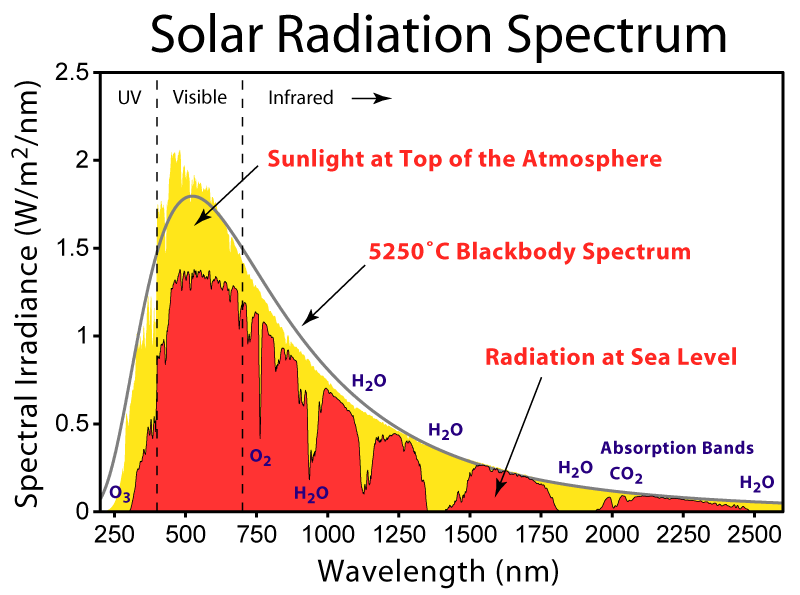
\includegraphics[width=0.7\textwidth]{Solar_Spectrum}
	\caption{Spektrum der Sonne. Sonnenlicht nehmen wir als weiß wahr.\\Quelle: https://commons.wikimedia.org/wiki/File:Solar\_Spectrum.png}
	\end{figure}

	\begin{figure}[h]
	\centering
	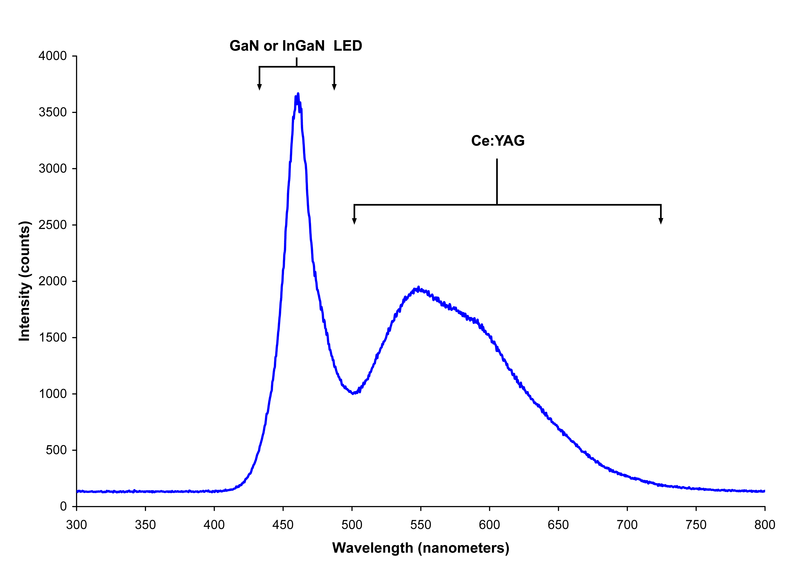
\includegraphics[width=0.7\textwidth]{White_LED}
	\caption{Spektrum einer weißen LED.\\Quelle: https://commons.wikimedia.org/wiki/File:White\_LED.png}
	\end{figure}

	\newpage
	
	\section{Lampen}
	\textbf{Schreiben Sie drei verschiedene Temperaturstrahler auf. Notieren Sie zu jedem die ungefähre Farbtemperatur.}\\
	\begin{itemize}
		\item \textbf{Wolframlampe}: ca 2500 bis 3500 Kelvin\\
		\item \textbf{Sonne}: ca 5500 Kelvin\\
		\item \textbf{Kerzenlicht}: ca 1000 bis 2000 Kelvin\\
	\end{itemize}
	Quelle: https://www.pixolum.com/blog/fotografie/weissabgleich-farbtemperatur\\
	
	\textbf{Schreiben Sie den Unterschied auf (ggf. mit kurzer Erläuterung) zwischen}\\
	\begin{itemize}
		\item \textbf{Lichtfarbe}: Die Farbe in der wir das Licht wahrnehmen.\\
		\item \textbf{Farbwiedergabe}: Wie viel des natürlich Spektrums abgedeckt ist.\\
		\item \textbf{Farbtemperatur}: Je wärmer ein Temperaturstrahler ist, umso bläulicher ist sein abgestrahltes Licht. Je höher die Farbtemperatur in Kelvin, umso "kälter" nehmen wir das Licht wahr.\\
	\end{itemize}
	
	\textbf{Erläutern Sie an Folie 41 ganz knapp, weshalb eine Glühlampe eine geringe Lichtausbeute hat.}\\
	Weil viel Leistung notwendig ist, bis der Glühdraht eine sichtbare Wellenlänge zu strahlen beginnt. Ein Großteil der erzeugten Strahlung liegt im Infrarotbereich und erzeugt somit Wärme.\\
	
	\textbf{Warum ist eine Halogenlampe besser, aber immer noch nicht gut?}\\
	Das Halogen verlängert die Lebensdauer, senkt aber nicht die notwendige Temperatur um Licht auszustrahlen.\\
	
	\textbf{Welchen Vorteil besitzen Entladungslampen gegenüber Temperaturstrahlern?}\\
	Leuchtstofflampen sind energieeffizienter, da nicht so viel Leistung in Hitze umgewandelt wird. Sie bieten außerdem eine höhere Lebensdauer da kein Glühdraht vorhanden ist welcher verdampft.\\
	
	\textbf{Welchen Nachteil besitzen Entladungslampen gegenüber Temperaturstrahlern?}\\
	Spezielle Elektronik wird zur Strombegrenzung benötigt.\\
	
	\newpage
	
	\textbf{Schreiben Sie eine Liste mit den drei Lampenarten. Schreiben Sie Vorteile und Nachteile jeweils auf.}\\
	\begin{center}
		\begin{tabular}{ c|c|c }
			& Vorteile & Nachteile \\ 
			\hline
			LED & Gute Lichtausbeute & Wellenlänge ändert sich mit der Zeit \\
			Entladungslampe & Lange Lebensdauer & Elektronik zur Strombegrenzung \\
			Temperaturstrahler & Sehr preiswert & Niedrige Lebensdauer, schlechte Lichtausbeute \\
		\end{tabular}
	\end{center}
	\vspace{10pt}
	
	\section{Hell- und Dunkelfeld}
	\textbf{Kurze Beschreibung Hell- und Dunkelfeld mit Einsatzgebieten.}\\
	\begin{center}
		\begin{tabular}{ c|c }
			 & Beschreibung \\ 
			\hline
			Hellfeld & Reflektiertes Licht scheint in die Kamera. \\
			& Typische Beleuchtung von Objekten.\\
			\hline
			Dunkelfeld & Kein reflektiertes Licht scheint in die Kamera.\\
			& Nur Streulicht wird von der Kamera eingefangen.\\
			& Einsatz häufig in der Oberflächeninspektion.\\
		\end{tabular}
	\end{center}
	\vspace{10pt}
	
	\section{Beleuchtung}
	\textbf{Schreiben Sie eine kleine Tabelle zum Thema Beleuchtung mit Vor- und Nachteilen.}\\
	\begin{center}
		\begin{tabular}{ c|c|c }
			& Vorteile & Nachteile \\ 
			\hline
			Weißes Licht & Deckt das sichtbare Spektrum ab & niedrigere Auflösung wgn Bayer Matrix\\
			Monochromatisch & Höhere Auflösung & Aufwändiger wenn Farbbilder benötigt \\
			\hline
			Gerichtetes Licht & Richtung ist bekannt & schwierig bei spiegelnden Oberflächen \\
			Diffuses Licht & gleichmäßige Beleuchtung & kein Dunkelfeld \\
			Linienlicht & Höhenprofil kann aufgenommen werden & Sehr spezieller Aufgabenbereich \\
		\end{tabular}
	\end{center}
	\vspace{10pt}
	
	\newpage
	
	\section{Spiegelnde Oberflächen}
	\textbf{Welche Probleme haben Sie bei der Beleuchtung von (leicht) spiegelnden Oberflächen?}\\
	Dass das licht eventuell nicht in die Kamera reflektiert wird, bzw. dass Spiegelungen auf der Oberfläche die Inspektion stören.
	\textbf{Nennen Sie grundsätzliche Lösungsmöglichkeiten, durch optische Maßnahmen, insbesondere bei der Beleuchtung, solche Probleme in den Griff zu bekommen?}\\
	Koaxiale Beleuchtung und/oder Polarisationsfilter um Reflektionen unter Kontrolle zu bringen.
	Spiegelung zu Nutze machen, zB. bei Fehlersuche mit Dunkelfeld.
	
	\section{Getaktete Beleuchtung}
	\textbf{Können sie sich vorstellen, welche Vorteile getaktete Beleuchtung haben kann?}\\
	Eine getaktete Beleuchtung ermöglicht es schnelle Bewegungen einzufrieren. Außerdem können mehrere Bilder mit verschiedenen Beleuchtungen gemacht werden (Beispiel: gerichtete Beleuchtung aus verschiedenen Richtungen, um Oberflächendefekte zu finden).

	
\end{document}
